\chapter{Sistemas de Unidades de Medidas}
O Sistema Métrico é um sistema internacional de medições que determina as unidades a serem utilizadas por cada uma das medidas, além de suas transformações. A unidade fundamental desse sistema é o metro ($m$), porém, cada medida tem sua unidade padrão, de acordo com o Sistema Internacional de Unidades.

\section{Medidas de comprimento}
As medidas de comprimento são os mecanismos de medição mais utilizados. A unidade fundamental das medidas de comprimento é o metro ($m$). 
\begin{multicols}{2}
	\subsection{Múltiplos de metro}
		\begin{itemize}
			\item Quilômetro $(km) = 1000m = 10^3m$
			\item Hectômetro $(hm) = 100m = 10^2m$
			\item Decâmetro $(dam) = 10m$ 
			
		\end{itemize}

	\subsection{Submúltiplos de metro}
		\begin{itemize}
			\item Decimetro $(dm) = 0,1m = 10^{-1}m$
			\item centímetro $(cm) = 0,01m = 10^{-2}m$
			\item Milímetro $(mm) = 0,001m = 10^{-3}m$
		\end{itemize}
\columnbreak
     \bigskip
     \noindent   % Very important in case that \parindent is not 0pt
     \begin{minipage}{\linewidth}
            \centering 
            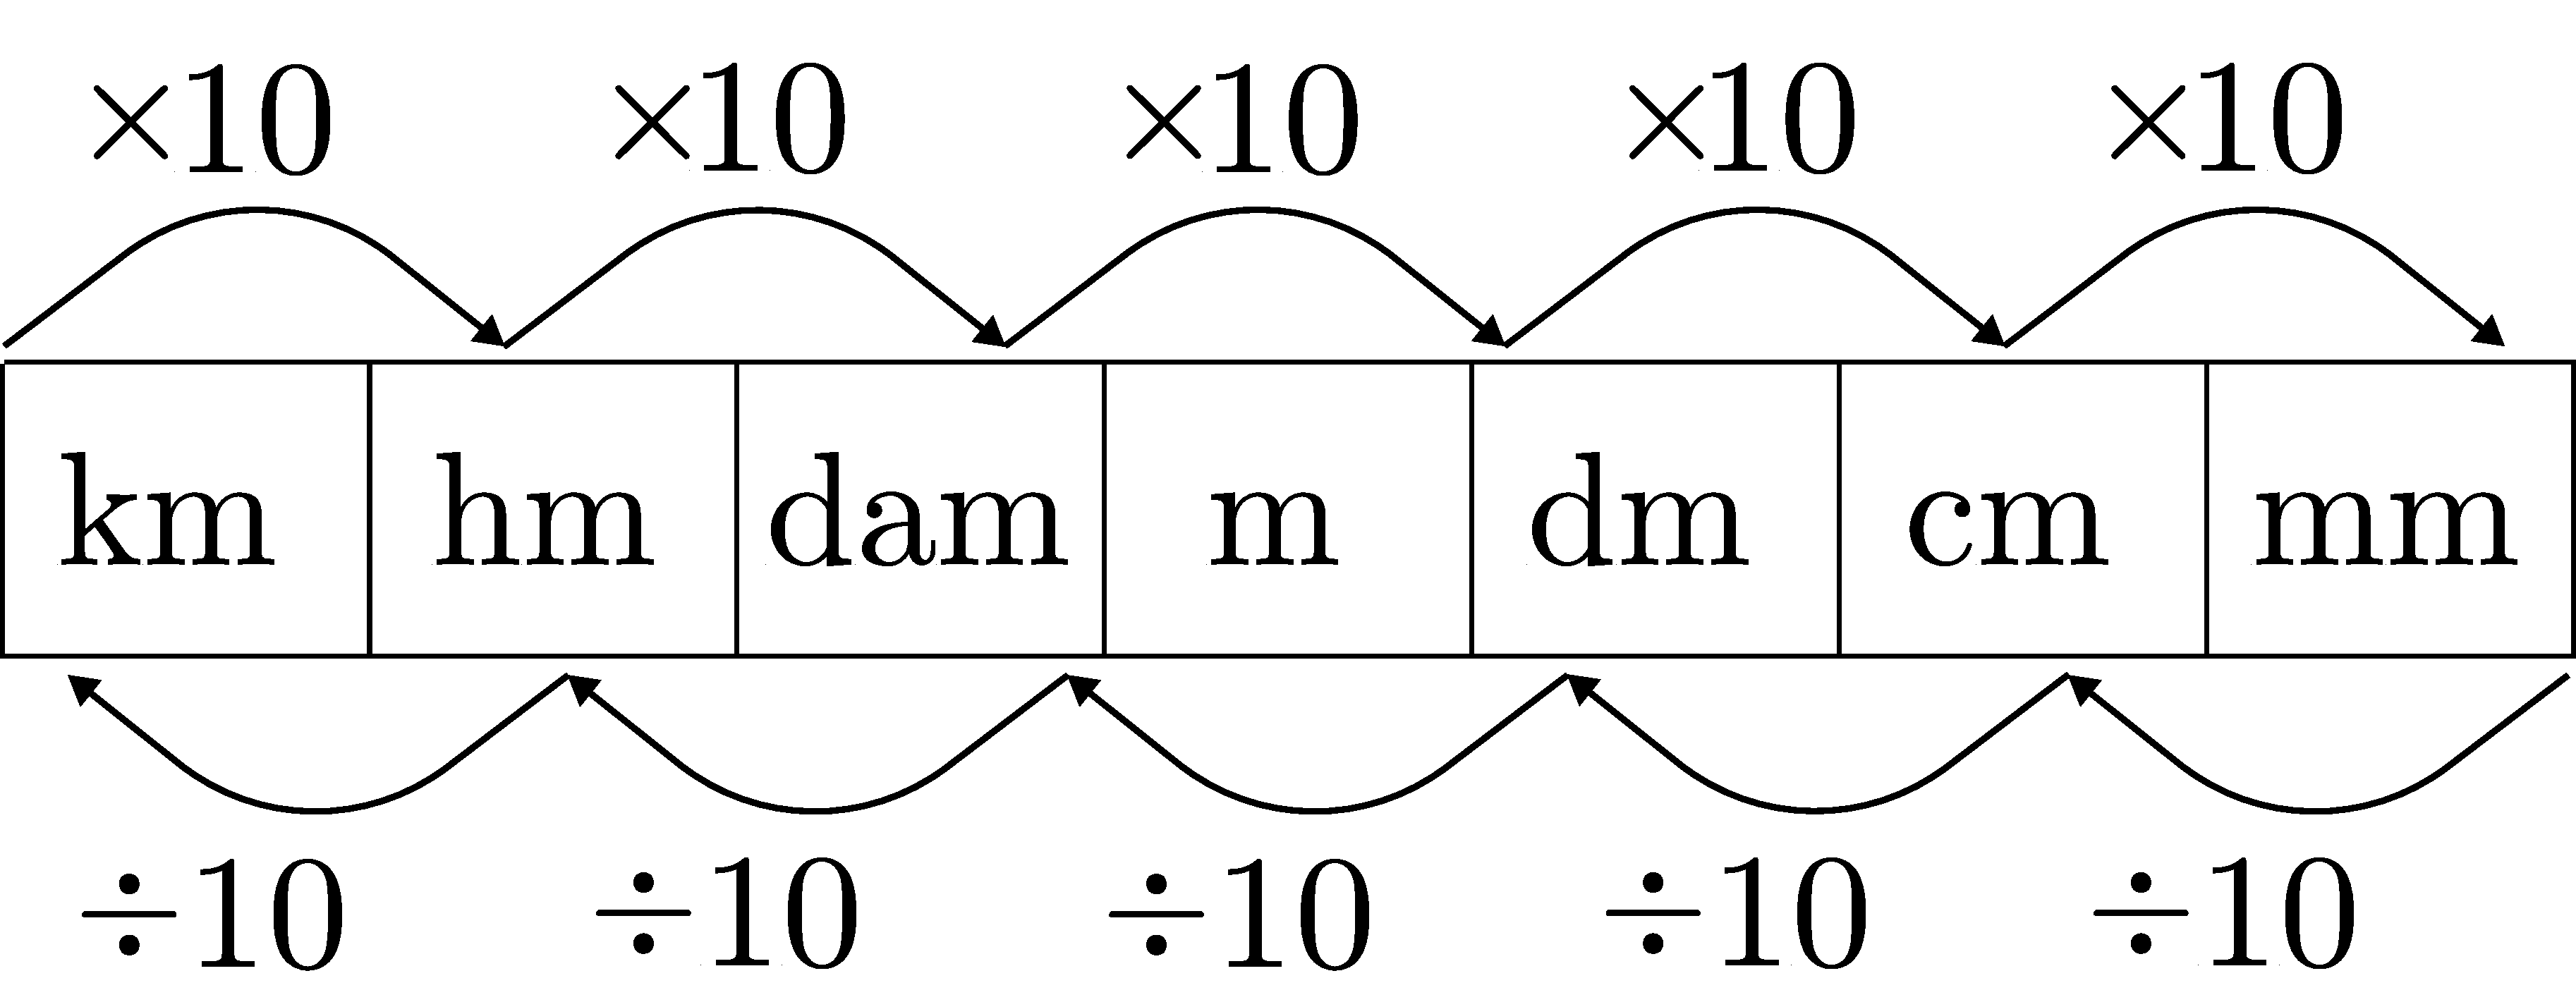
\includegraphics[width=0.8\textwidth]{imagens/matematicaBasica/sistemaDeUnidades/MultiplosDeMetro.pdf}
             \label{figura:MultiplosDeMetro}
       \captionof{figure}{Múltiplos de metro}
     \end{minipage}
   \end{multicols}


\section{Medidas de Superfície}
As medidas de superfície são as utilizadas na medição de
áreas. Sua unidade fundamental é o metro quadrado ($m^2$).
    \subsection{Múltiplos de metro quadrado($m^2$)}
		\begin{itemize}
			\item Quilômetro quadrado $(km^2) = 1.000.000 m^2 = 10^6 m^2$
			\item Hectômetro quadrado $(hm^2) = 10.000 m^2 = 10^4 m^2$
			\item Decâmetro quadrado $(dam^2) = 100 m^2 = 10^2 m^2$
		\end{itemize}

	\subsection{Submúltiplos de metro quadrado}
		\begin{itemize}
			\item Decímetro quadrado $(dm^2) = 0,01m^2 = 10^{-2}m^2$
			\item centímetro quadrado $(cm^2) = 0,0001m^2 = 10^{-4}m^2$
			\item Milímetro quadrado $(mm^2)= 0,000001m^2 = 10^{-6}m^2$
		\end{itemize}

\section{Medidas Agrárias}
Dentre as medidas de superfícies, existem as medidas
agrárias, que são mais utilizadas para medir áreas rurais. Sua
unidade fundamental é o are ($a$).
	\begin{itemize}
		\item Centiare $(ca) = 1m^2=10^0m^2$
		\item Are $(a)= 100m^2 = 10^2m^2$
		\item Hectare $(ha) = 10000m^2 = 10^4m^2$
	\end{itemize}

\section{Medidas de Volume} 
As medidas de volume são utilizadas $g$ para medir o espaço ocupado por um corpo tridimensional ou a sua capacidade de armazenar alguma
substância. Em química, as medidas de volume geralmente aparecem quando medimos quantidades de líquidos. A unidade métrica tradicional de volume usada nesse caso é o litro (L). Em termos
do SI, um litro é definido exatamente como $14 decímetro cúbico$.

\subsection{Múltiplos do Metro Cubico:}
		\begin{itemize}
		    \item Quilômetro cúbico $(Km^3) = 1.000.000.000 m^3 = 10^9 m^3$
		    \item Hectômetro cúbico $(hm^3) = 1.000.000 m^3 = 10^6 m^3$
		    \item Decâmetro cúbico $(dam^3) = 1.000 m^3 = 10^3 m^3$
		\end{itemize}
	
\subsection{Submúltiplos de metros cúbicos $(m^3)$}
		\begin{itemize}
		    \item Decímetro cúbico $(dm^3) = 0,001 m^3 = 10^{-3} m^3$
		    \item Centímetro cúbico $(cm^3) = 0,000001 m^3 = 10^{-6} m^3$
		    \item Milímetro cúbico $(mm^3) = 0,000000001 m^3 = 10^{-9} m^3$
		\end{itemize}
		
		\begin{figure}
		    \centering 
            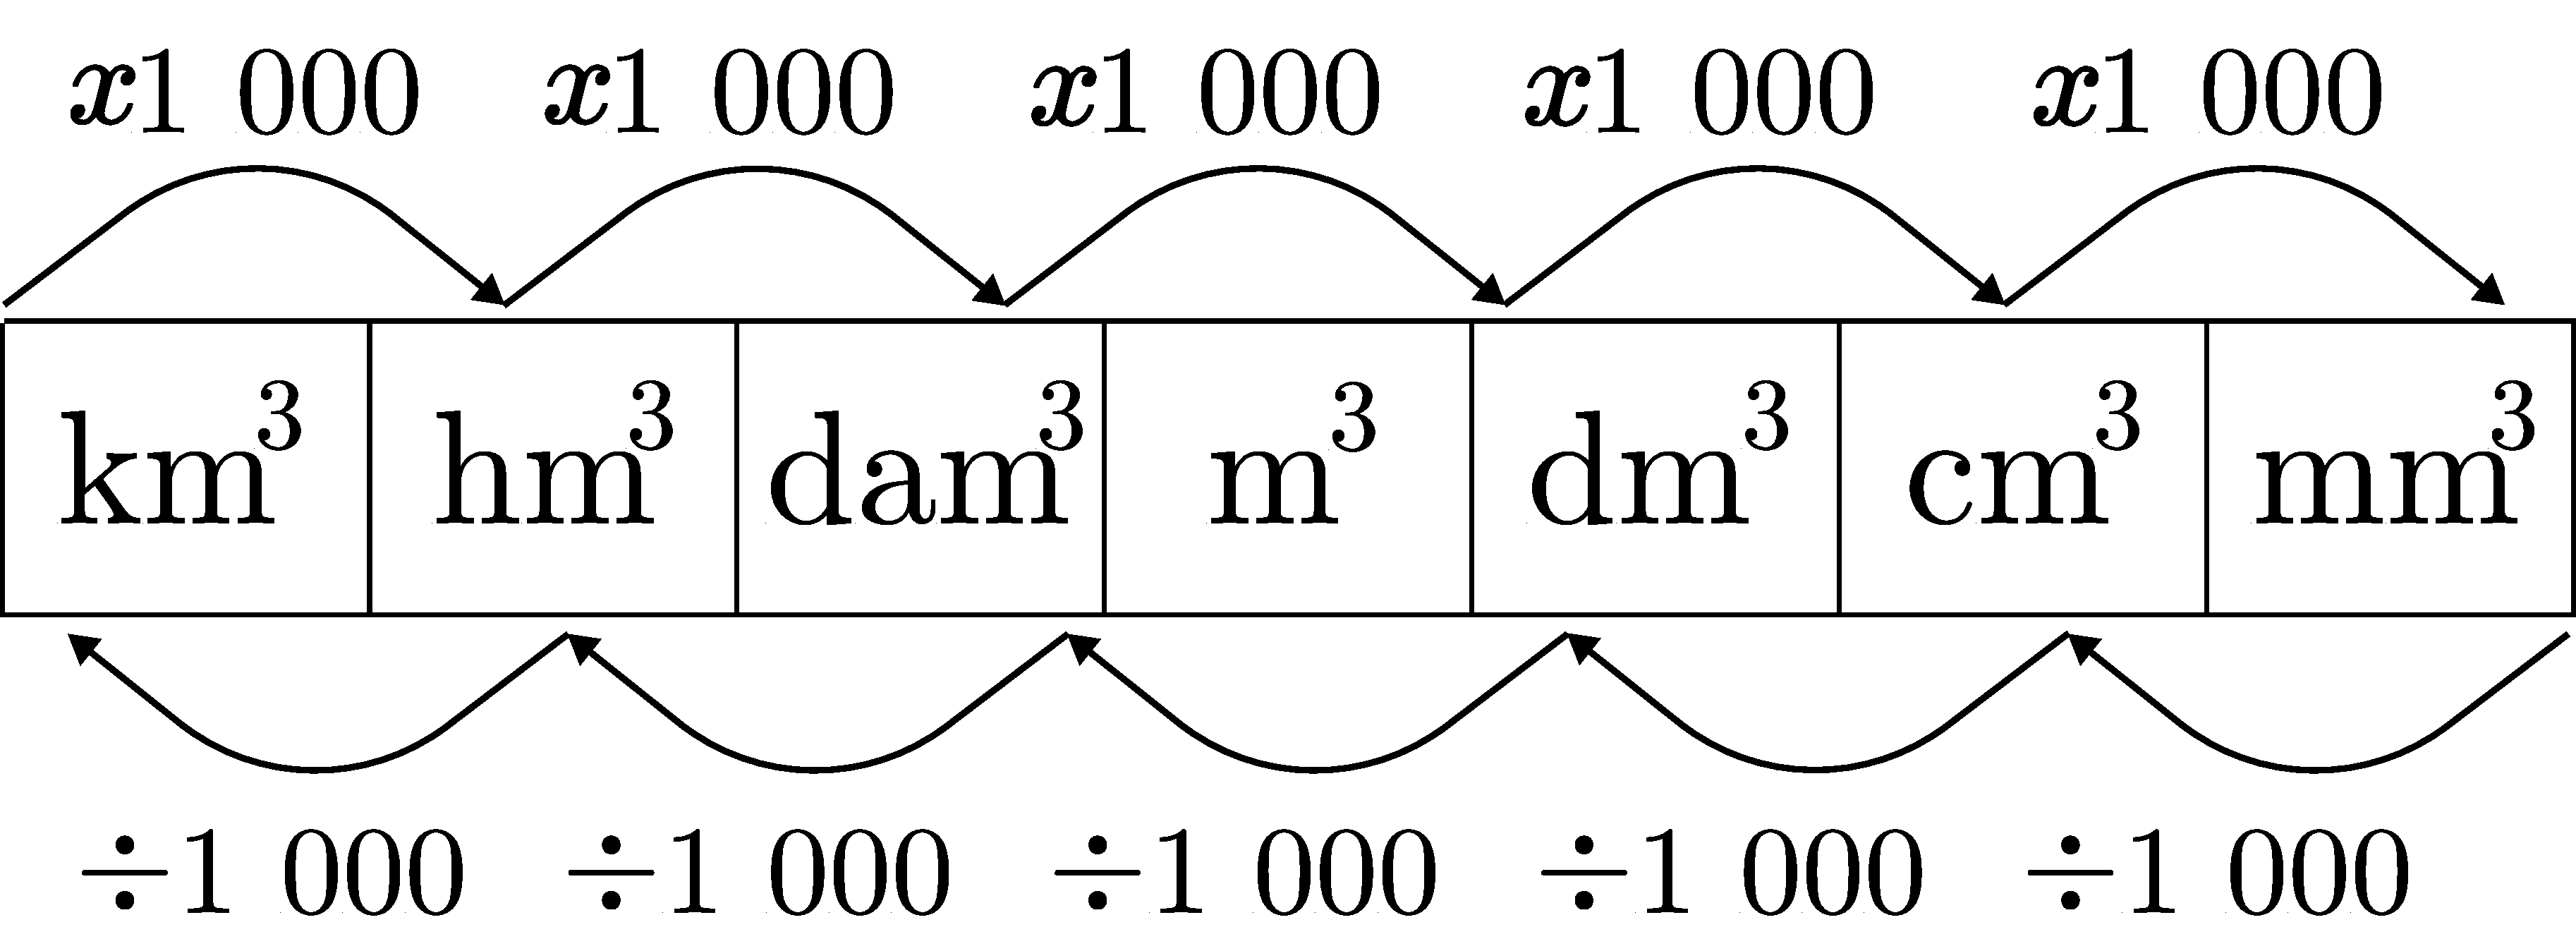
\includegraphics[width=0.4\textwidth]{imagens/matematicaBasica/sistemaDeUnidades/MultiplosDeMetroCubico.pdf}
		    \caption{Múltiplos de metro cubico}
		\end{figure}
     
\section{Medidas de Capacidade}
As medidas de capacidade são utilizadas para representarem
as grandezas que definem o volume contido em um certo
reservatório. A mais utilizada é o litro ($l$).
	\\\textbf{Importante:}
	\begin{itemize}
	    \item $1l = 1dm^3$
	    \item $1 ml = 1 cm^3$
	    \item $10^3 l = 1 m^3$
	\end{itemize}
\begin{multicols}{2}
	\subsection{Múltiplos de litro:}
		\begin{itemize}
		    \item Quilolitro $(Kl) = 1000 l = 10^3 l$
		    \item Hectolitro $(hl) = 100 l = 10^3 l$
		    \item Decalitro $(dal) = 10 l = 10^1l$
		\end{itemize}
	
	\subsection{Submúltiplos de Litro:}
		\begin{itemize}
		    \item Decilitro $(dl) = 0,1 l = 10^{-1}l$
		    \item Centilitro $(cl) = 0,01 l = 10^{-2}l$
		    \item Mililitro $(ml) = 0,001 l = 10^{-3}l$
		\end{itemize}
\columnbreak
     \bigskip
     \noindent   % Very important in case that \parindent is not 0pt
     \begin{minipage}{\linewidth}

    \centering 
    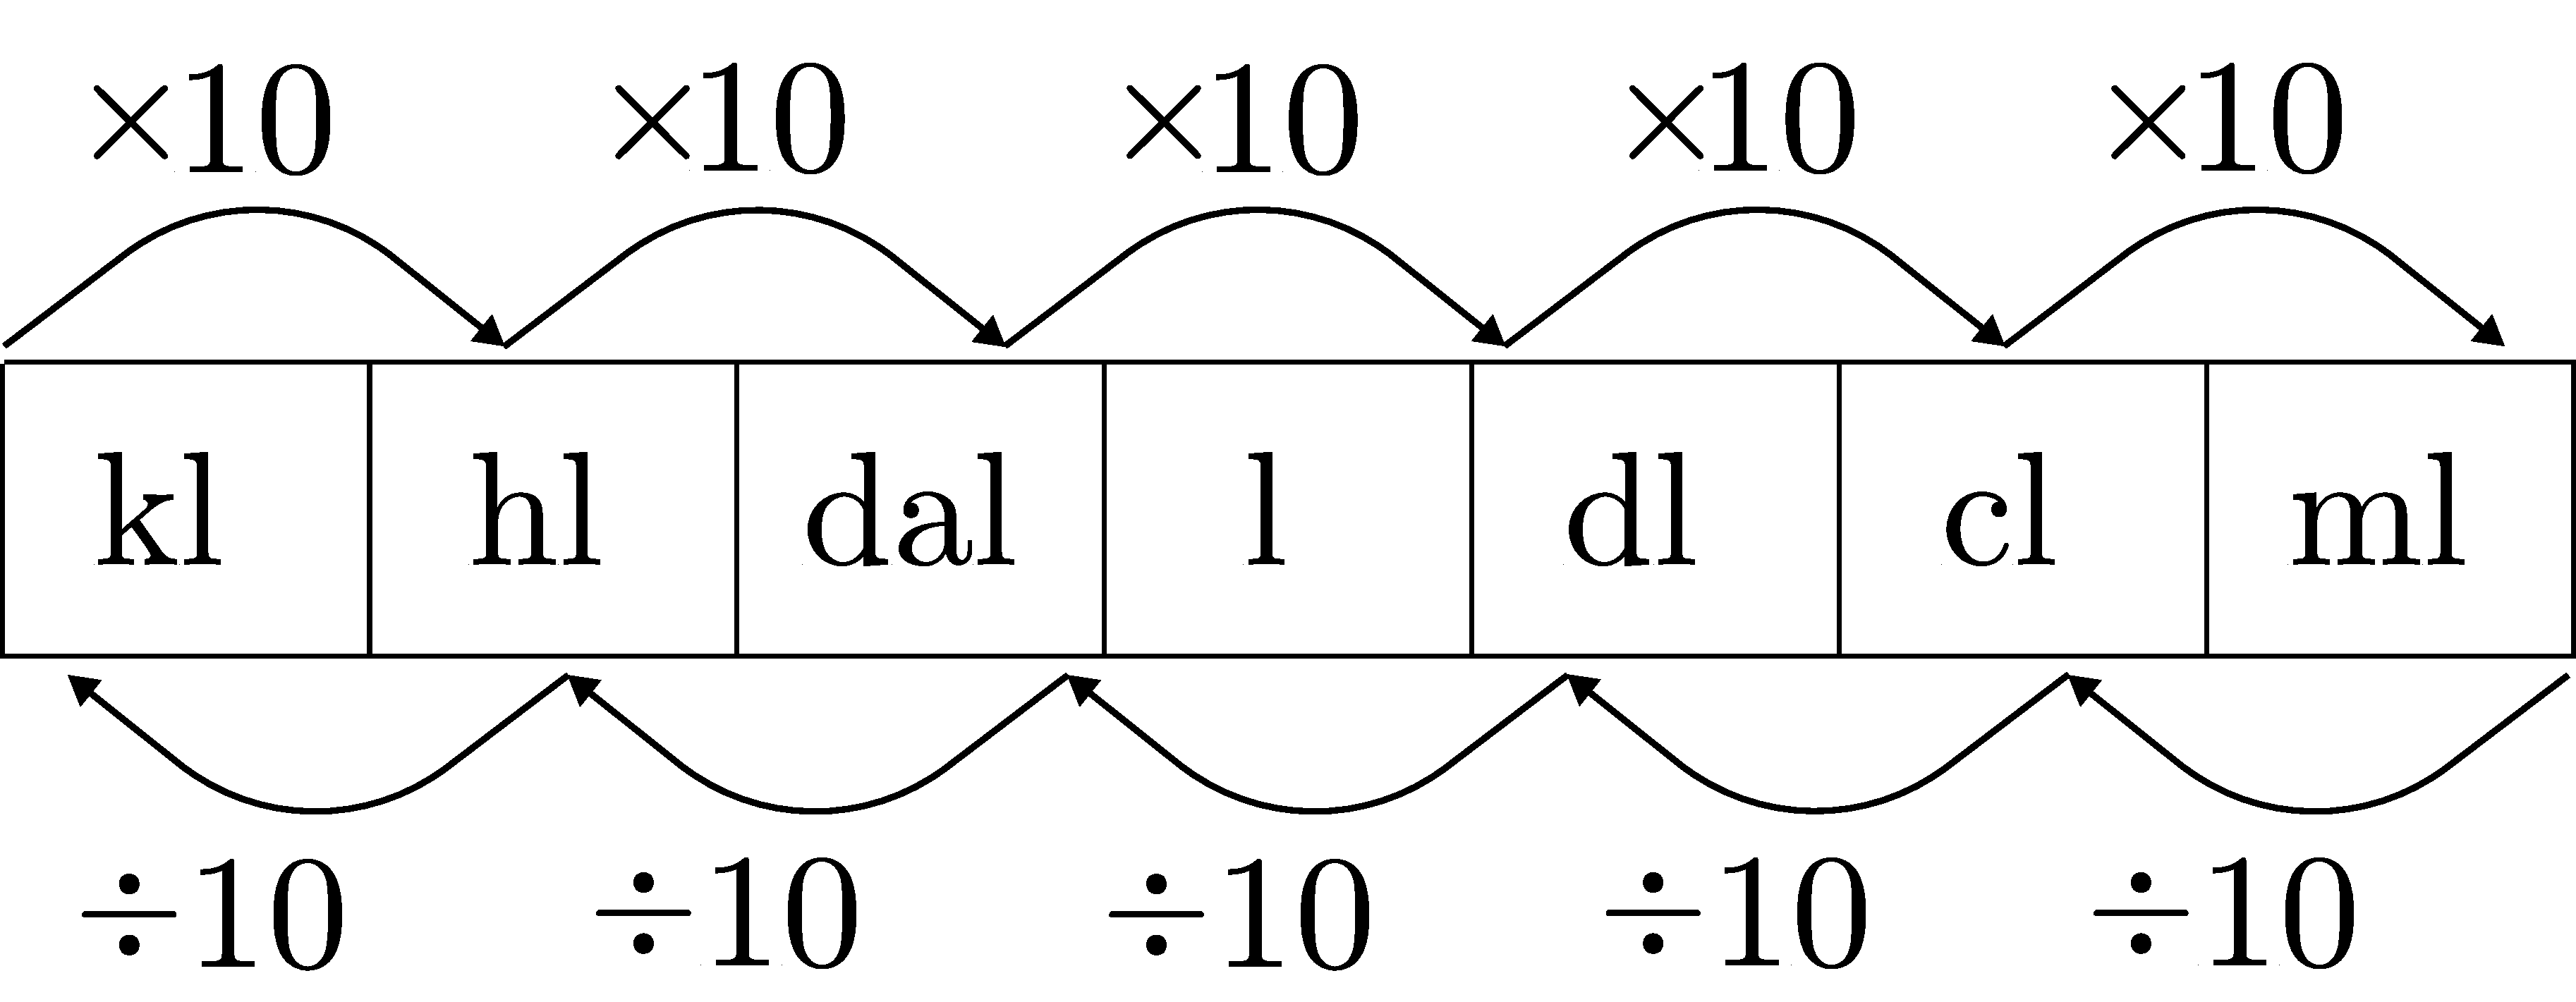
\includegraphics[width=0.8\textwidth]{imagens/matematicaBasica/sistemaDeUnidades/MultiplosDeLitro.pdf}
   \captionof{figure}{Múltiplos de litro}
     \end{minipage}
   \end{multicols}  

\section{Medidas de Massa}
As medidas de massa são utilizadas para medir a quantidade
de massa em um corpo. No SI, a unidade fundamental de massa é
o quilograma ($kg$), embora o grama ($g$) seja a unidade mais
conveniente para a maioria das medidas de laboratório.
\begin{multicols}{2}
	\subsection{Múltiplos de Grama:}
		\begin{itemize}
		    \item Quilograma $(Kg) = 1000 g = 10^3 g$
		    \item Hectograma $(hg) = 100 g = 10^2 g$
		    \item Decagrama $(dag) = 10 g = 10^1 g$
		\end{itemize}
	
	\subsection{Submúltiplos de Grama:}
		\begin{itemize}
		    \item Decigrama $(dg) = 0,1 g = 10^{-1} g$
		    \item Centigrama $(cg) = 0,01 g = 10^{-2} g$
		    \item Miligrama $(mg) = 0,001 g = 10^{-3}$
		\end{itemize}
		\columnbreak
     \bigskip
     \noindent   % Very important in case that \parindent is not 0pt
     \begin{minipage}{\linewidth}
    \centering 
    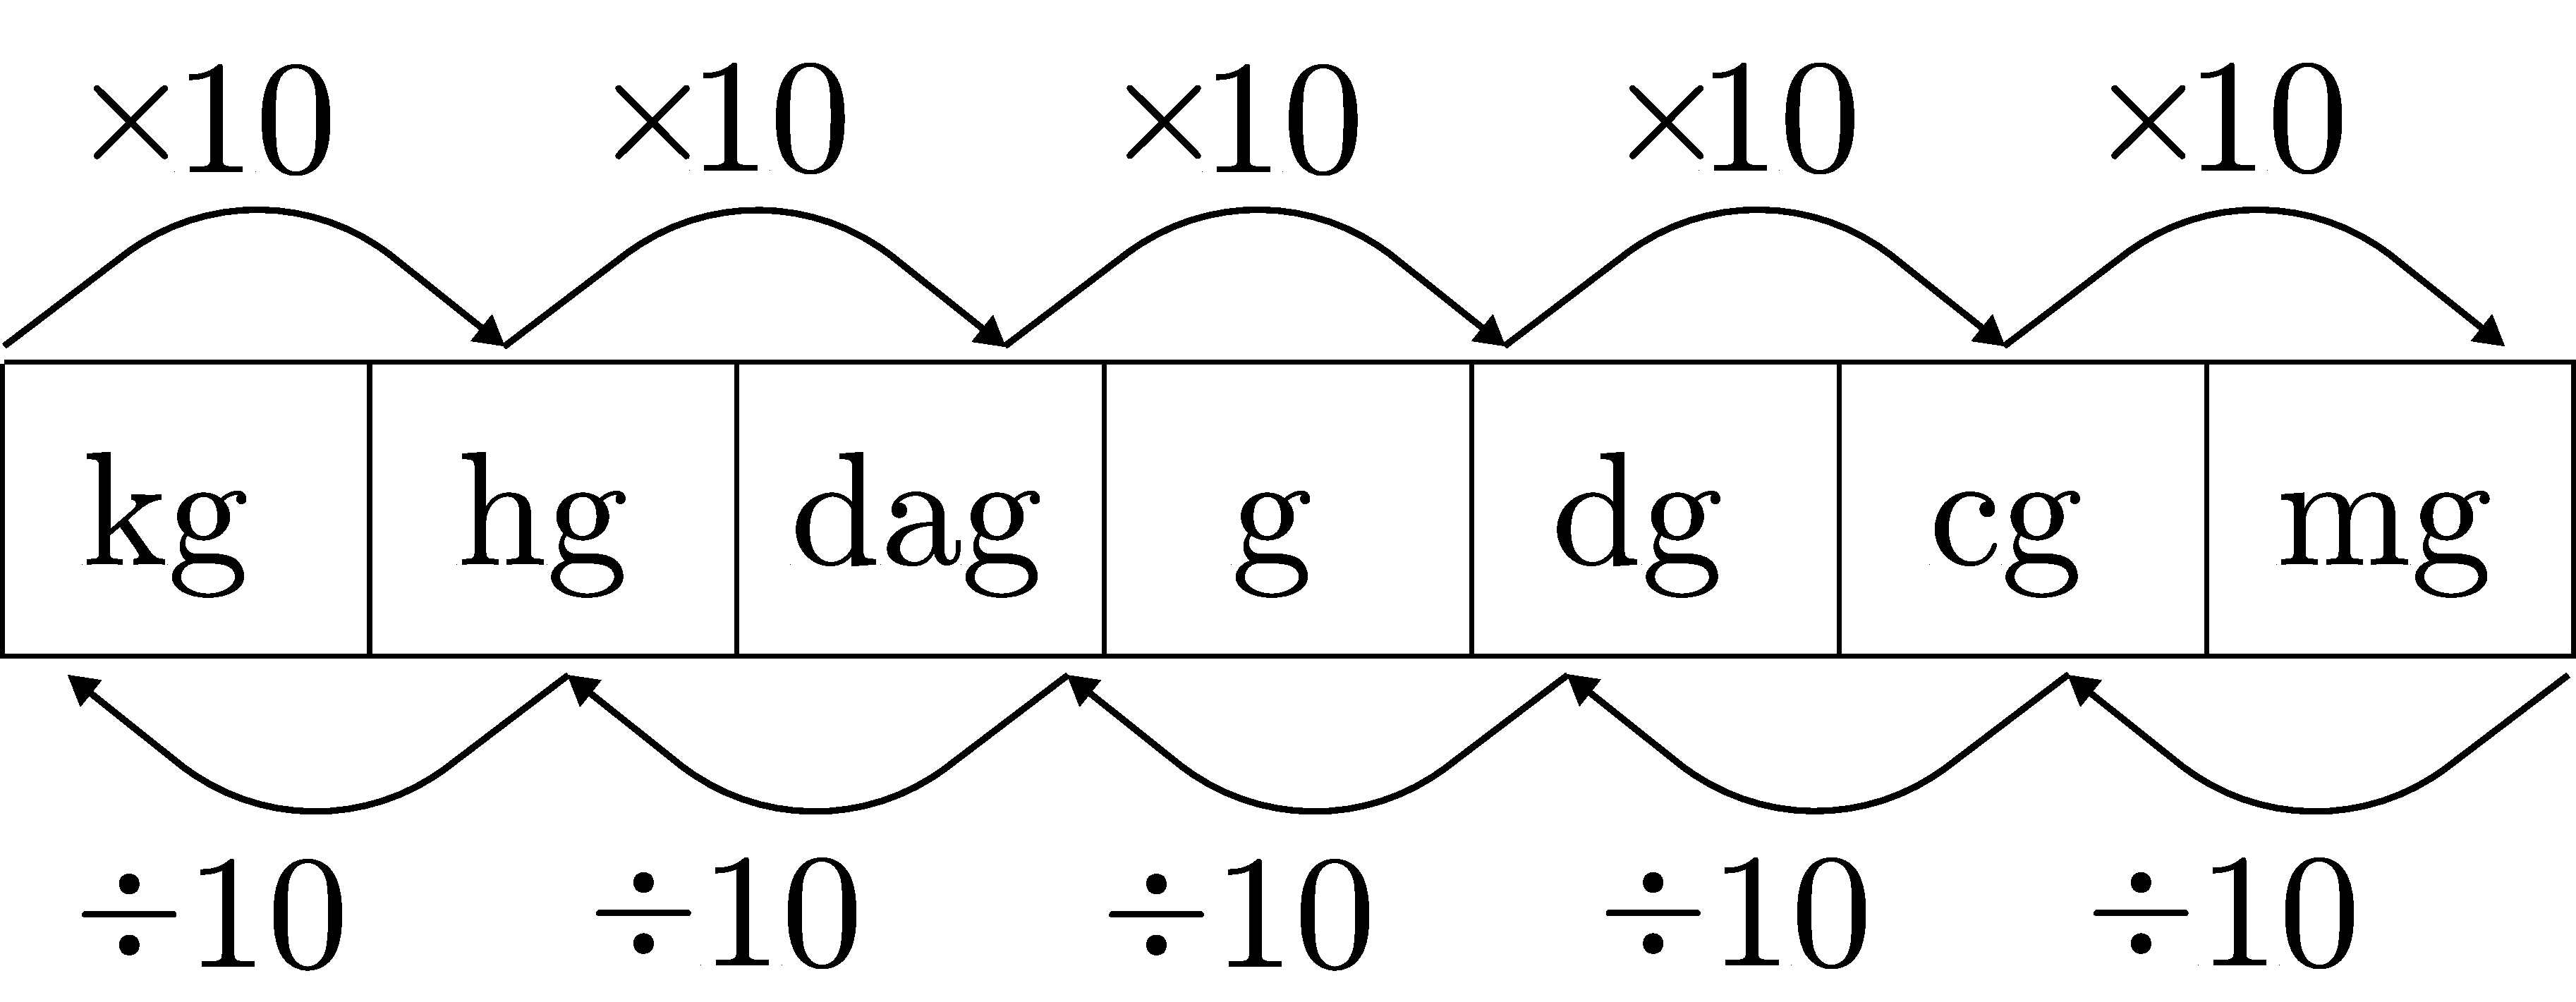
\includegraphics[width=0.8\textwidth]{imagens/matematicaBasica/sistemaDeUnidades/MultiplosDeGrama.pdf}
    \captionof{figure}{Múltiplos de grama}
\end{minipage}
   \end{multicols} 
Existe ainda a unidade especial:
Tonelada $(t) = 1000 kg = 10^3 kg = 10^6 g$

\section{Exercícios}

	\begin{exercise}[ENEM 2017]
	Uma empresa especializada em conservação de piscinas utiliza um produto para tratamento da água cujas especificações técnicas sugerem que seja adicionado 1,5 ml desse produto para cada 1000 l de água da piscina. Essa empresa foi contratada para cuidar de uma piscina de base retangular, de profundidade constante igual a 1,7 m, com largura e comprimento iguais a 3 m e 5 m, respectivamente. O nível da lâmina d’água dessa piscina é mantido a 50 cm da borda da piscina.

A quantidade desse produto, em mililitro, que deve ser adicionada a essa piscina de modo a atender às suas especificações técnicas é :
    \begin{description}
        \item[a)] $11,25$
        \item[b)] $27,00$
        \item[c)] $28,80$
        \item[d)] $32,25$
        \item[e)] $49,50$
    \end{description}
\end{exercise}

\begin{exercise}[ENEM 2010]
Um consumidor desconfia que a balança do supermercado não está aferindo corretamente a massa dos produtos. Ao chegar a casa resolve conferir se a balança estava descalibrada. Para isso, utiliza um recipiente provido de escala volumétrica, contendo $1,0$ litro d’água. Ele coloca uma porção dos legumes que comprou dentro do recipiente e observa que a água atinge a marca de $1,5$ litro e também que a porção não ficara totalmente submersa, com $1/3$ de seu volume fora d’água. Para concluir o teste, o consumidor, com ajuda da internet, verifica que a  densidade dos legumes, em questão, é a metade da densidade da água, onde, $ \rho \cdot \textrm{água} = 1 g/cm^{3}$.

No supermercado a balança registrou a massa da porção de legumes igual a $0,500 kg$ (meio quilograma).Considerando que o método adotado tenha boa precisão, o consumidor concluiu que a balança estava descalibrada e deveria ter registrado a massa da porção de legumes igual a:

    \begin{description}
        \item[a)] $0,073~kg$
        \item[b)] $0,167~kg$
        \item[c)] $0,250~kg$
        \item[d)] $0,375~kg$
        \item[e)] $0,750~kg$
    \end{description}
\end{exercise}
	
\newpage
\begin{figure}[!h]
    \centering
    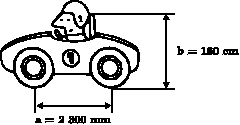
\includegraphics[width=0.5\textwidth]{imagens/matematicaBasica/sistemaDeUnidades/carro.pdf}
\end{figure}
\begin{exercise}[ENEM 2011]
Um mecânico de uma equipe de corrida necessita que as seguintes medidas realizadas em um carro sejam obtidas em metros: a) distância a entre os eixos dianteiro e traseiro;

Ao optar pelas medidas $a$ e $b$ em metros, obtêm-se, respectivamente,

    \begin{description}
        \item[a)] $0,23 \textrm{ e } 0,16$
        \item[b)] $2,3 \textrm{ e } 1,6$
        \item[c)] $23 \textrm{ e } 16$
        \item[d)] $230 \textrm{ e } 160g$
        \item[e)] $2300 \textrm{ e } 1600$
    \end{description}

\end{exercise}

\begin{exercise}[ENEM 2011]
Um aluno de Ensino Médio vai até o açougue, a pedido de seus pais, comprar $5 kg$ de carne para um churrasco em sua casa. Além da carne, ele compra $8$ litros de refrigerante para oferecer aos convidados. Qual das alternativas a seguir possui os valores da quantidade de carne e de refrigerante, respectivamente, nas unidades tonelada $(t)$ e mililitro $(ml)$?

    \begin{description}
        \item[a)] $0,005 t e 0,008 ml$
        \item[b)] $5000 t e 0,008 ml$
        \item[c)] $0,005 t e 8000 ml$
        \item[d)] $5000 t e 8000 ml$
        \item[e)] $0,005 t e 0,8 ml$
    \end{description}

\end{exercise}
\begin{exercise}[ENEM 2011]


    \begin{description}
        \item[a)] $0,23 \textrm{ e } 0,16$
        \item[b)] $2,3 \textrm{ e } 1,6$
        \item[c)] $23 \textrm{ e } 16$
        \item[d)] $230 \textrm{ e } 160g$
        \item[e)] $2300 \textrm{ e } 1600$
    \end{description}

\end{exercise}